\subsubsection{Fine-tuning methodology for RoBERTa}

To fine-tune the pretrained \texttt{twitter-roBERTa} model and adapt it to solve the classification task, we used the tokenized input data, which had not yet been embedded by the model. These data were split into 70\%, 15\%, and 15\% for the training, validation, and test sets, respectively, similar to the BI-LSTM architecture. 

Next, we created a three-layer classification head following the architecture shown in Figure~\ref{fig:roberta_finetune_architecture}. Dropout layers were added to prevent overfitting. This classification head was then integrated with the RoBERTa encoder, using the representation of the \texttt{[CLS]} token, which, as mentioned before, summarizes the input sequence.

With the full model ready, we froze the RoBERTa weights to train only the classification head. The training lasted 150 epochs, used batches of 32 samples, and employed the Adam optimizer, storing the checkpoints of the best-performing models. After this first stage, we evaluated the results and performed a second training stage, where all pretrained weights were unfrozen. This second stage was trained using a learning rate of 0.000001, the Adam optimizer, for 100 epochs, again with a batch size of 32.

To assess the best model from each training stage as well as the untrained model, we used precision, recall, F1-score, accuracy, and the confusion matrix.

\begin{figure}[htbp]
  \centering
  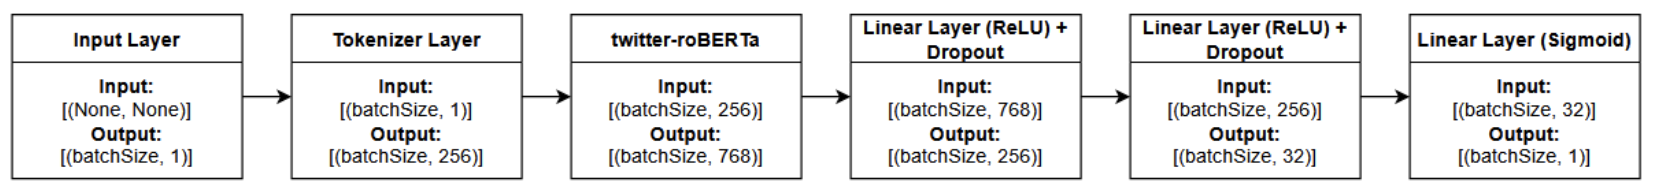
\includegraphics[width=0.45\textwidth]{images/roberta_finetune_architecture.png}
  \caption{Architecture used for fine-tuning twitter-RoBERTa.}
  \label{fig:roberta_finetune_architecture}
\end{figure}
